\ProvidesFile{ch-introduction.tex}[2022-10-05 introduction chapter]

\chapter{INTRODUCTION}



Single molecule localization microscopy (SMLM) relies on the temporal resolution of fluorophores in the sample whose spatially overlapping point spread functions would otherwise render them unresolvable at the detector. SMLM techniques, such as stochastic optical reconstruction microsscopy (STORM) and photo-activated localization microscopy (PALM) remain desirable for super-resolution imaging of many cellular structures, due to their cost-effective implementation and diffraction unlimited resolution (Schermelleh 2019). Common strategies for the temporal separation of molecules involve transient intramolecular rearrangements to switch from dark to fluorescent states or the exploitation of non-emitting molecular radicals. For direct STORM (dSTORM), rhodamine derivatives can undergo intersystem crossing to a triplet state, which can be reduced by thiols to form a dark radical species. The dark state can then be quenched by oxidative processes, driving the fluorophore back to its ground state (Figure 1a). Long dark state lifetimes are commonly used in STORM imaging in order to maintain sparse activation and high resolution.

\subsection{The definition of resolution in SMLM}

The distribution of a particular biomolecule in the cell can be described as a probability density over a two-dimensional space, casting super-resolution as a density estimation problem. Intuitively, the spatial resolution of SMLM images then increases as we draw more samples from this density - a concept which is made mathematically precise by the so-called Fourier ring correlation or FRC. Using FRC, one can compute image resolution as the spatial frequency at which a correlation function in the frequency domain drops below a threshold, typically taken to be $1/7$ (See Supplement). According to this theory, reducing localization uncertainty while increasing the number of samples, results in an increase in image resolution (Nieuwenhuizen 2013). However, there remains a fundamental limit to the the minimal localization uncertainty which can be obtained.

\begin{figure}
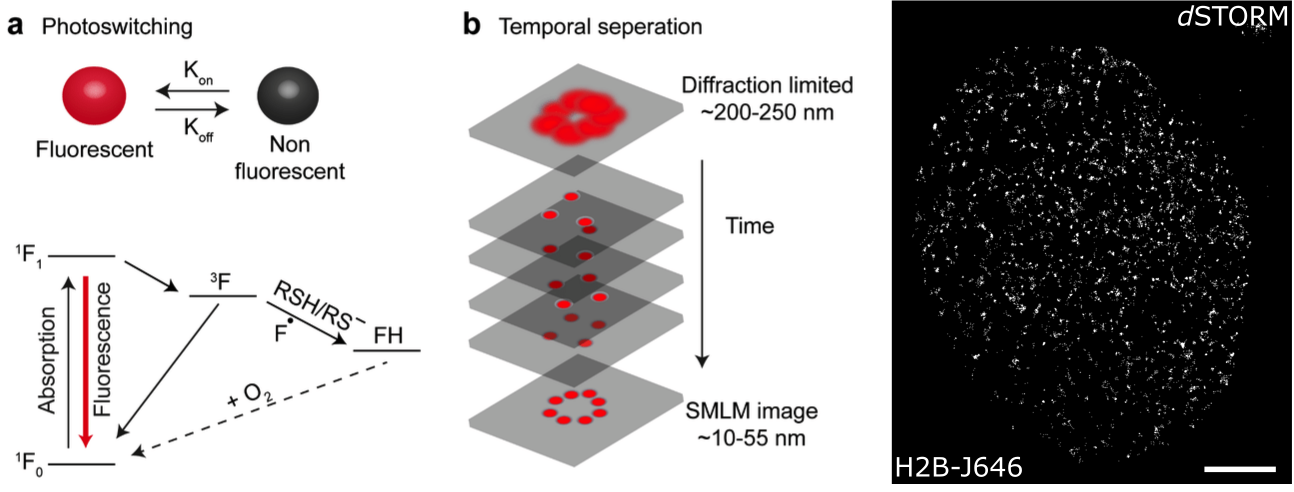
\includegraphics[width=\textwidth]{figures/Intro.png}
\caption{\textbf{Stochastic optical reconstruction microscopy (STORM)}. (A) Single molecules are resolved by separating their fluorescent emission in time, using fluorophores with multiple photophysical states (B) Example super-resolution image of H2B protein in a living Hela cell nucleus at 37C, 5 percent CO2. Image reconstructed from $10^{3}$ 10ms frames. Scalebar 5um.}
\end{figure}

Localization uncertainty, typically the RMSE of a maximum likelihood or similar statistical estimator, is bounded from below by the inverse of the Fisher information matrix, known as the Cramer-Rao lower bound (Chao 2016). Localization uncertainties in sparse conditions are often tens of nanometers, although recent work on integration of Bayesian priors with modulation enhanced SMLM (meSMLM) or structured illumination with MINFLUX, has reduced spatial resolution below to a few nanometers (Kalisvaart 2022, Gwosh 2020). Nevertheless, managing the increase in localization uncertainty at high labeling density remains a major bottleneck to SMLM. Static uncertainty due to molecular crowding can be partially amelioriated by using pairwise or higher-order temporal correlations within a pixel neighborhood, known as stochastic optical fluctuation imaging or SOFI (Dertinger 2009). Other approaches such as stimulated emission and depletion (STED) imaging bring control over the photophysical state of a chosen subset of the sample, yet the need for laser scanning prevents widespread application in live-cell studies. The spatial resolution and relative simplicity of SMLM techniques remains unmatched, inciting an effort to increase the resolution of SMLM techniques and explore avenues towards time resolved SMLM.

\subsection{Novel contributions to the field}

Here, we present single photon counting enhanced SMLM and a technique for super-resolution imaging of chromatin nanodomains in-vivo. We address dense SMLM by utilizing a high-speed single photon avalanche diode (SPAD) camera. SPAD cameras provide the necessary functionality for both single molecule localization and counting. Then, we present a more conventional dSTORM approach to study spatial organization of nucleosomes in living cells, with a particular focus on the structure of phase separated condensates containing bromodomain protein 4 (BRD4) protein.


